% Generated from ../chapters/16-endogenous-escape-velocity.md
\chapter{Chapter 16 --- Endogenous Escape Velocity}\label{chapter-16-endogenous-escape-velocity}

Suppose damage burden is \(D(t)\) and adaptive reserve is \(R(t)\). A minimal model is

\[
\frac{dD}{dt}=g(D,t)-c(R,D),
\]

\[
\frac{dR}{dt}=aL-bL^2+sS-rD-\mu R.
\]

Here \(g\) is new damage generation, \(c\) is clearance and repair, \(L\) is adaptive loading, \(S\) is recovery support such as sleep and nourishment, and the negative \(bL^2\) term represents overload. Damage reduces reserve; reserve can improve repair.

The model is conceptual, but unlike a decorative equation it yields interpretable behaviour. If loading is zero, reserve may decay through disuse. If loading is excessive, overload dominates. At intermediate load, reserve grows. If higher reserve increases clearance, the system can enter a virtuous loop. If damage suppresses reserve strongly, it enters a vicious loop.

\begin{figure}
\centering
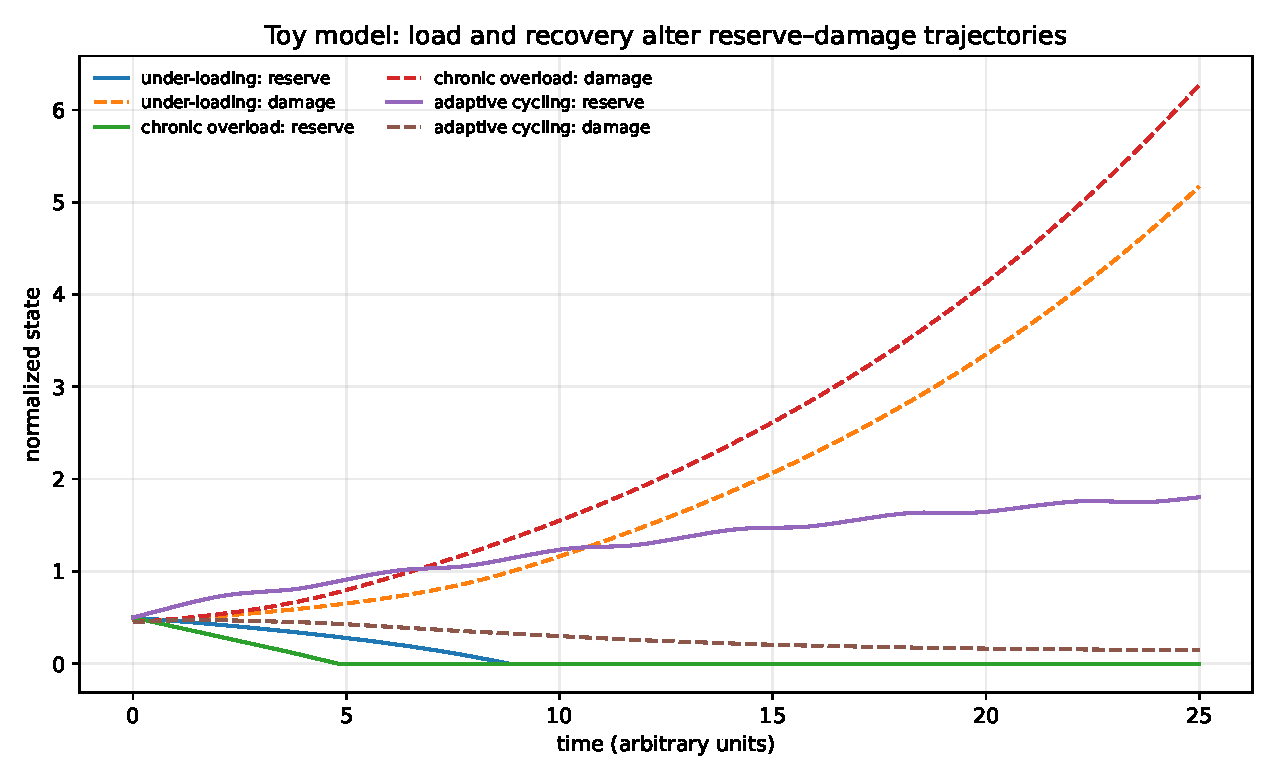
\includegraphics[width=0.88\textwidth]{../figures/reserve-damage-trajectories-v4.pdf}
\caption{Conceptual trajectories of reserve and damage under under-loading, chronic overload, and adaptive cycling. The goal is not maximal stress but a regime in which reserve improves future clearance.}
\end{figure}

An escape threshold occurs when effective repair and clearance exceed new damage for long enough that reserve itself improves:

\[
c(R,D)>g(D,t), \qquad \frac{dR}{dt}>0.
\]

This does not imply exponential rejuvenation forever. Repair saturates, irreversibilities remain, and cancer constraints limit proliferation. A plausible trajectory is sigmoid: slow initial change, acceleration as constraints loosen, and a plateau near a new viable regime.

The distinctive claim is second-order. A successful cycle should not only improve the current state. It should improve \textbf{improvability}: the response to the next cycle.

This can be tested. After a period of intervention, expose the person to a standardized training, metabolic, or cognitive challenge. Does adaptation occur faster? Does recovery improve? Does the system tolerate a wider range without losing coherence?

Endogenous escape velocity is not currently demonstrated in humans. It is a research hypothesis built by applying de Grey's rate-based reasoning to internal adaptive dynamics.

\section{Reading the phase diagram}\label{reading-the-phase-diagram}

The model suggests four regimes. Low load and low recovery produce disuse. High load and low recovery produce breakdown. Moderate load and adequate recovery produce adaptation. High reserve and controlled load may produce a region where repair exceeds damage.

The boundary between regimes is not fixed. Age, disease, genetics, and history change it. A training dose adaptive at thirty may be destructive at seventy unless recovery and progression are adjusted.

\section{Why positive feedback need not mirror negative feedback}\label{why-positive-feedback-need-not-mirror-negative-feedback}

Your symmetry argument is conceptually strong: if declining function reduces future repair, improving function can improve future repair. But the loops are not equal because biological ceilings, irreversible loss, and cancer suppression create asymmetry. The question is not whether perfect symmetry exists but whether the positive region is larger than current practice assumes.
